\documentclass{article}

\usepackage{amsmath,amssymb}
\usepackage{tikz}
\usepackage{pgfplots}
\usepackage{xcolor}
\usepackage[left=2.1cm,right=3.1cm,bottom=3cm,footskip=0.75cm,headsep=0.5cm]{geometry}
\usepackage{enumerate}
\usepackage{enumitem}
\usepackage{marvosym}
\usepackage{tabularx}
\usepackage{parskip}

\usepackage{listings}
\definecolor{lightlightgray}{rgb}{0.95,0.95,0.95}
\definecolor{lila}{rgb}{0.8,0,0.8}
\definecolor{mygray}{rgb}{0.5,0.5,0.5}
\definecolor{mygreen}{rgb}{0,0.8,0.26}
%\lstdefinestyle{java} {language=java}
\lstset{language=R,
	basicstyle=\ttfamily,
	keywordstyle=\color{lila},
	commentstyle=\color{lightgray},
	stringstyle=\color{mygreen}\ttfamily,
	backgroundcolor=\color{white},
	showstringspaces=false,
	numbers=left,
	numbersep=10pt,
	numberstyle=\color{mygray}\ttfamily,
	identifierstyle=\color{blue},
	xleftmargin=.1\textwidth, 
	%xrightmargin=.1\textwidth,
	escapechar=§,
	%literate={\t}{{\ }}1
	breaklines=true,
	postbreak=\mbox{\space}
}

\usepackage[colorlinks = true, linkcolor = blue, urlcolor  = blue, citecolor = blue, anchorcolor = blue]{hyperref}
\usepackage[utf8]{inputenc}

\renewcommand*{\arraystretch}{1.4}

\newcolumntype{L}[1]{>{\raggedright\arraybackslash}p{#1}}
\newcolumntype{R}[1]{>{\raggedleft\arraybackslash}p{#1}}
\newcolumntype{C}[1]{>{\centering\let\newline\\\arraybackslash\hspace{0pt}}m{#1}}

\newcommand{\E}{\mathbb{E}}
\DeclareMathOperator{\rk}{rk}
\DeclareMathOperator{\Var}{Var}
\DeclareMathOperator{\Cov}{Cov}

\title{\textbf{Scalable Data Engineering, Exercise 1}}
\author{\textsc{Henry Haustein}}
\date{}

\begin{document}
	\maketitle
	
	\section*{Task 1}
	\begin{enumerate}[label=(\alph*)]
		\item False
		\item False
		\item False (?) it just provided a link to the data sources
		\item True
		\item False. The data cube is the base just for MOLAP. ROLAP uses a relational database.
		\item False. Depends on your goals/data.
		\item True
		\item False. It can have multiple fact tables.
		\item False. You have to transform it back to a data cube for better readability.
		\item True. If properly normalised.
	\end{enumerate}

	\section*{Task 2}
	\begin{center}
		\begin{tabular}{c|c|c}
			& one fact table & multiple fact tables \\
			\hline
			partially normalised & star schema & galaxy schema \\
			\hline
			normalised & snowflake schema & snowstorm schema
		\end{tabular}
	\end{center}
	
	\section*{Task 3}
	\begin{center}
		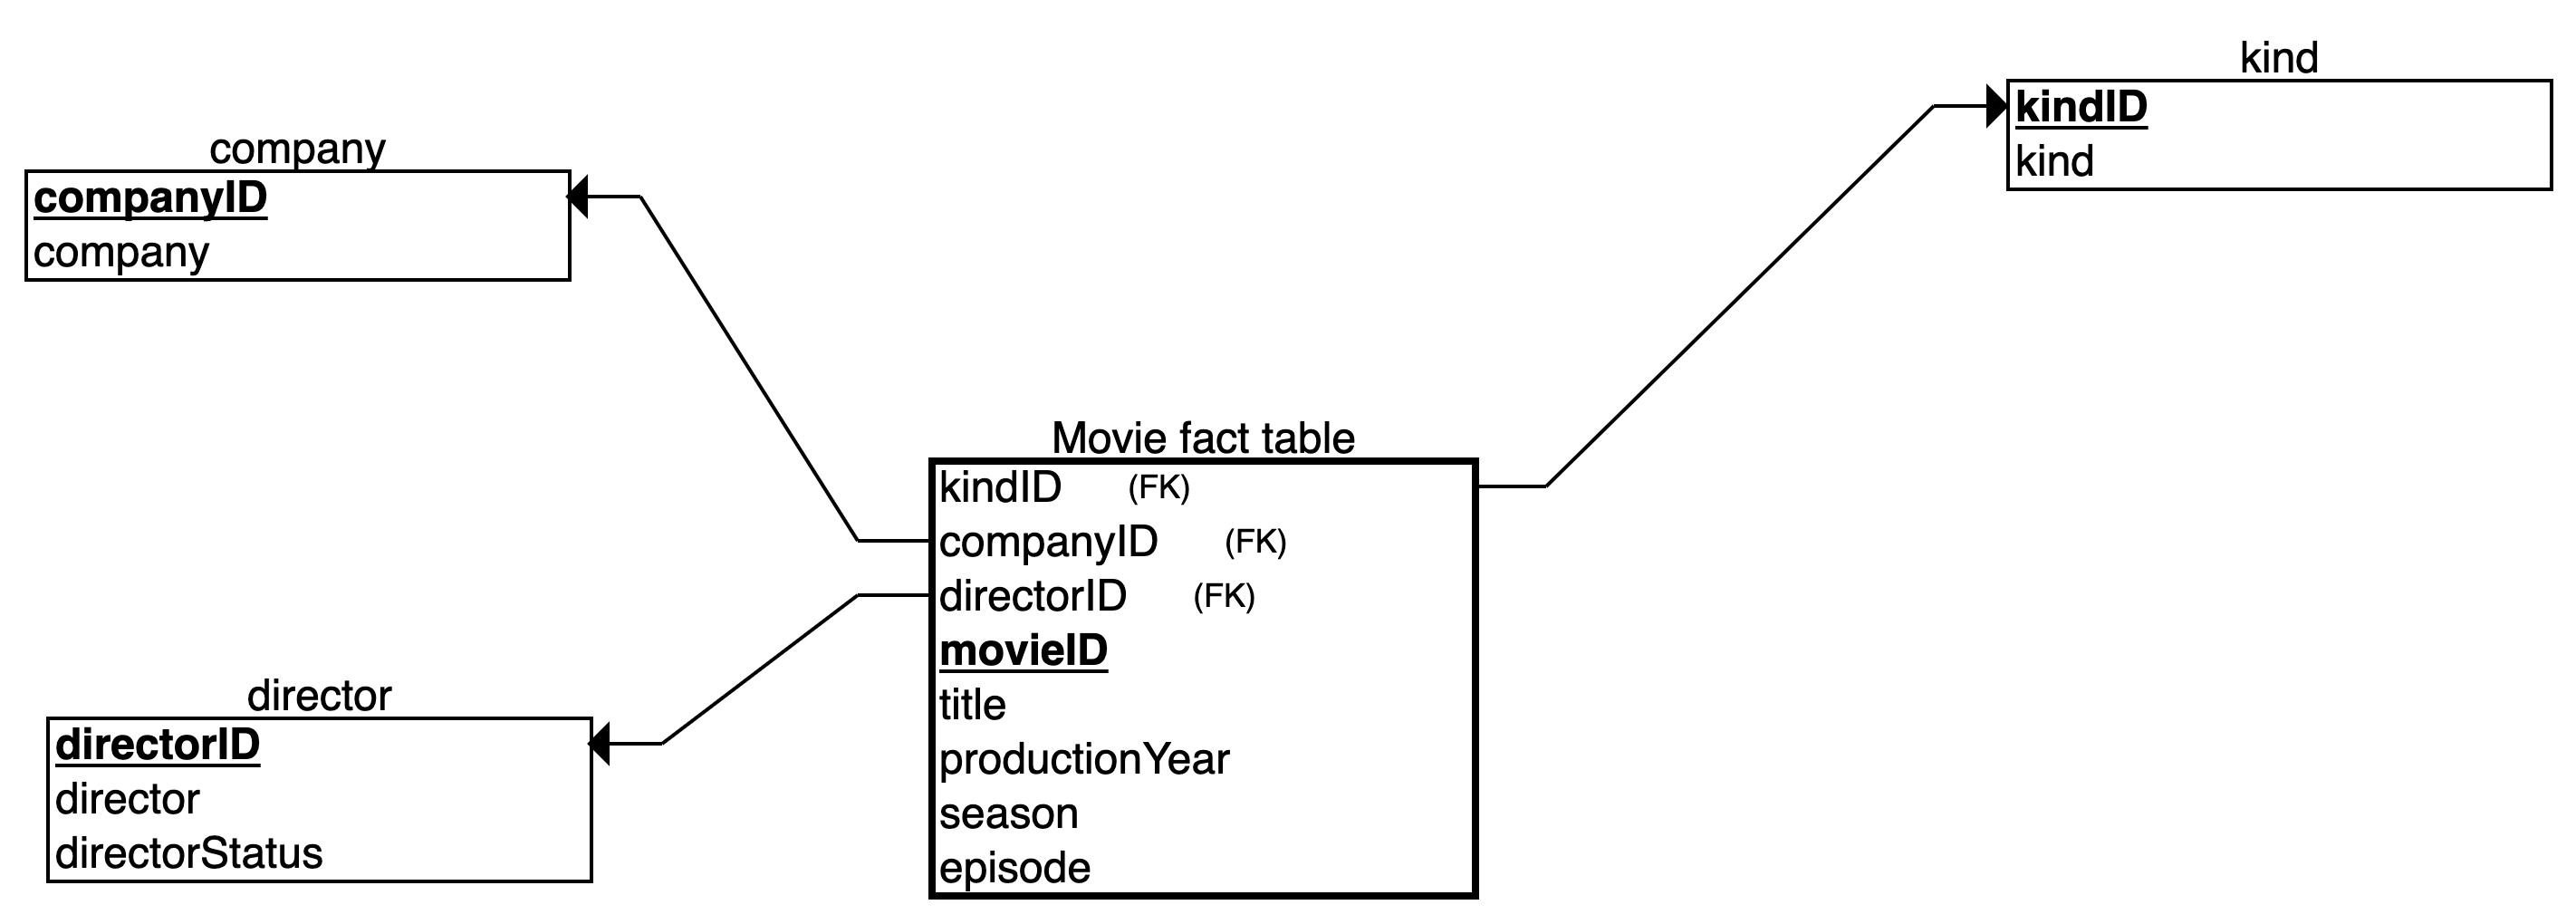
\includegraphics[scale=0.15]{task1.3}
	\end{center}
	
	\section*{Task 4}
	\begin{center}
		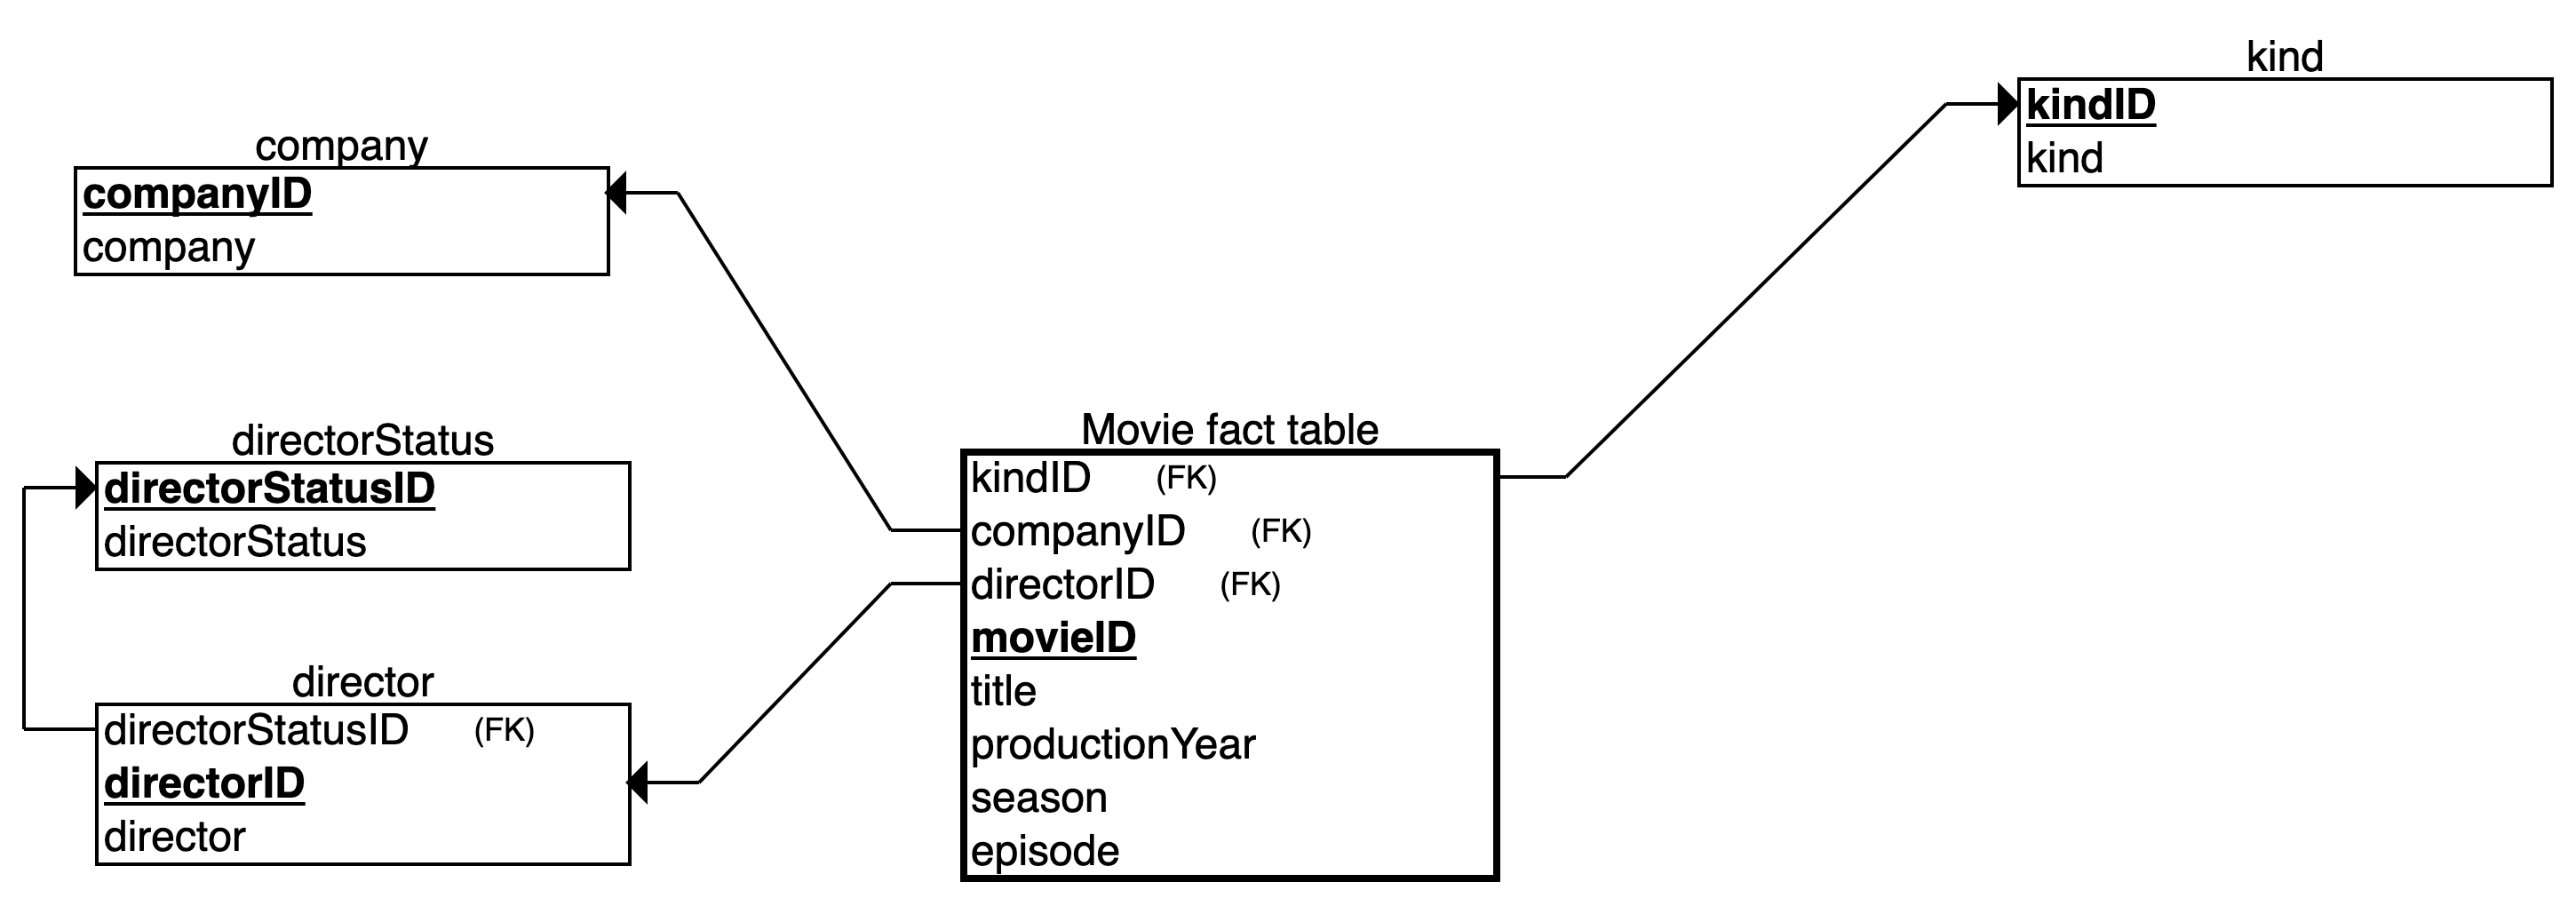
\includegraphics[scale=0.15]{task1.4}
	\end{center}
	
	\section*{Task 5}
	When storing all information in a single large table, each tuple (= row) consists of 5 strings and 1 integer, so in total $5\cdot 128\cdot 8\text{ Bit} + 3\cdot 64\text{ Bit} = 5.312\text{ Bit}$. With 1000 rows in this table, we need in total 5.312.000 Bit = 664.000 Byte. \textit{In the exercise they say the season and episode columns are empty, but we need to save them anyway.}
	
	For the star schema we have 4 tables:
	\begin{itemize}
		\item fact table: $1000\cdot (7\cdot 64\text{ Bit} + 128\cdot 8\text{ Bit}) = 1.472.000\text{ Bit}$
		\item company table: $1000\cdot (64\text{ Bit} + 128\cdot 8\text{ Bit}) = 1.088.000\text{ Bit}$
		\item director table: $1000\cdot (64\text{ Bit} + 2\cdot 128\cdot 8\text{ Bit}) = 2.112.000\text{ Bit}$
		\item kind table: $7\cdot (64\text{ Bit} + 128\cdot 8\text{ Bit}) = 7.616\text{ Bit}$
	\end{itemize}
	In total this are 4.679.616 Bit = 584.952 Byte.
	
	For the snowflake schema we have 5 tables:
	\begin{itemize}
		\item fact table: $1000\cdot (7\cdot 64\text{ Bit} + 128\cdot 8\text{ Bit}) = 1.472.000\text{ Bit}$
		\item company table: $1000\cdot (64\text{ Bit} + 128\cdot 8\text{ Bit}) = 1.088.000\text{ Bit}$
		\item director table: $1000\cdot (2\cdot 64\text{ Bit} + 128\cdot 8\text{ Bit}) = 1.152.000\text{ Bit}$
		\item director status table: $3\cdot (64\text{ Bit} + 128\cdot 8\text{ Bit}) = 3.264\text{ Bit}$
		\item kind table: $7\cdot (64\text{ Bit} + 128\cdot 8\text{ Bit}) = 7.616\text{ Bit}$
	\end{itemize}
	In total this are 3.722.880 Bit = 465.360 Byte.

\end{document}